\definecolor{dkgreen}{rgb}{0,0.6,0}
\definecolor{gray}{rgb}{0.5,0.5,0.5}
\definecolor{mauve}{rgb}{0.58,0,0.82}

\chapter{Testing}
\section{Testing Methodology}

For the testing of the protocol, we implemented a proof-of-concept in Python, using the OpenFHE library\cite{openFHE}. The testing methodology consists of the following steps. Firstly, we generate a set of random positions for the parking spots. After that, we generate a random position for the client, we compute the z-order encoding for both the client and the parking spots, and finally we computed the distances between the client position and the parking spots using the homomorphic encryption scheme.

To ensure a fair comparison, we test different scenarios with different sets of hyper parameters, such as the number of parking spots, the number of clients running simultaneously, a range of network delays, and the edge size in meters of a grid cell (used to encode the GPS coordinates). The goal is to measure the performance of the homomorphic encryption scheme in terms of encryption and decryption time, as well as the time taken to compute the distances between the client position and the parking spots.

At the same time, we also computed the distance calculation using a clear computation (trusted backend) with encrypted with asymmetric encryption (RSA) traffic. This allows us to compare the performance of the homomorphic encryption scheme against a traditional asymmetric encryption scheme.

The testing environment consists of a virtual machine instance on a server, with the following specifications:
\begin{itemize}
    \item CPU: Intel(R) Xeon(R) Silver 4110 CPU @ 2.10GHz 16 cores
    \item RAM: 64 GB
    \item OS: Debian 11
    \item Python version: 3.8
    \item OpenFHE version: 1.3.0.0.20.4
    \item numpy version: 1.24.0
\end{itemize}

\section{Performance Evaluation} \label{sec:testing-performance}

The first test that we perform is to measure the time taken to encrypt and decrypt the client position using the homomorphic encryption scheme. The results are shown in Figure \ref{fig:testing-enc}. The time taken to encrypt around 50 parkings with the same key is around 0.5 seconds, while the time taken to decrypt the client position is around 0.2 seconds. This resoults that the homomorphic encryption scheme is efficient for this use case, but it still grows linearly with the number of data points.

\begin{figure}[h]
    \centering
    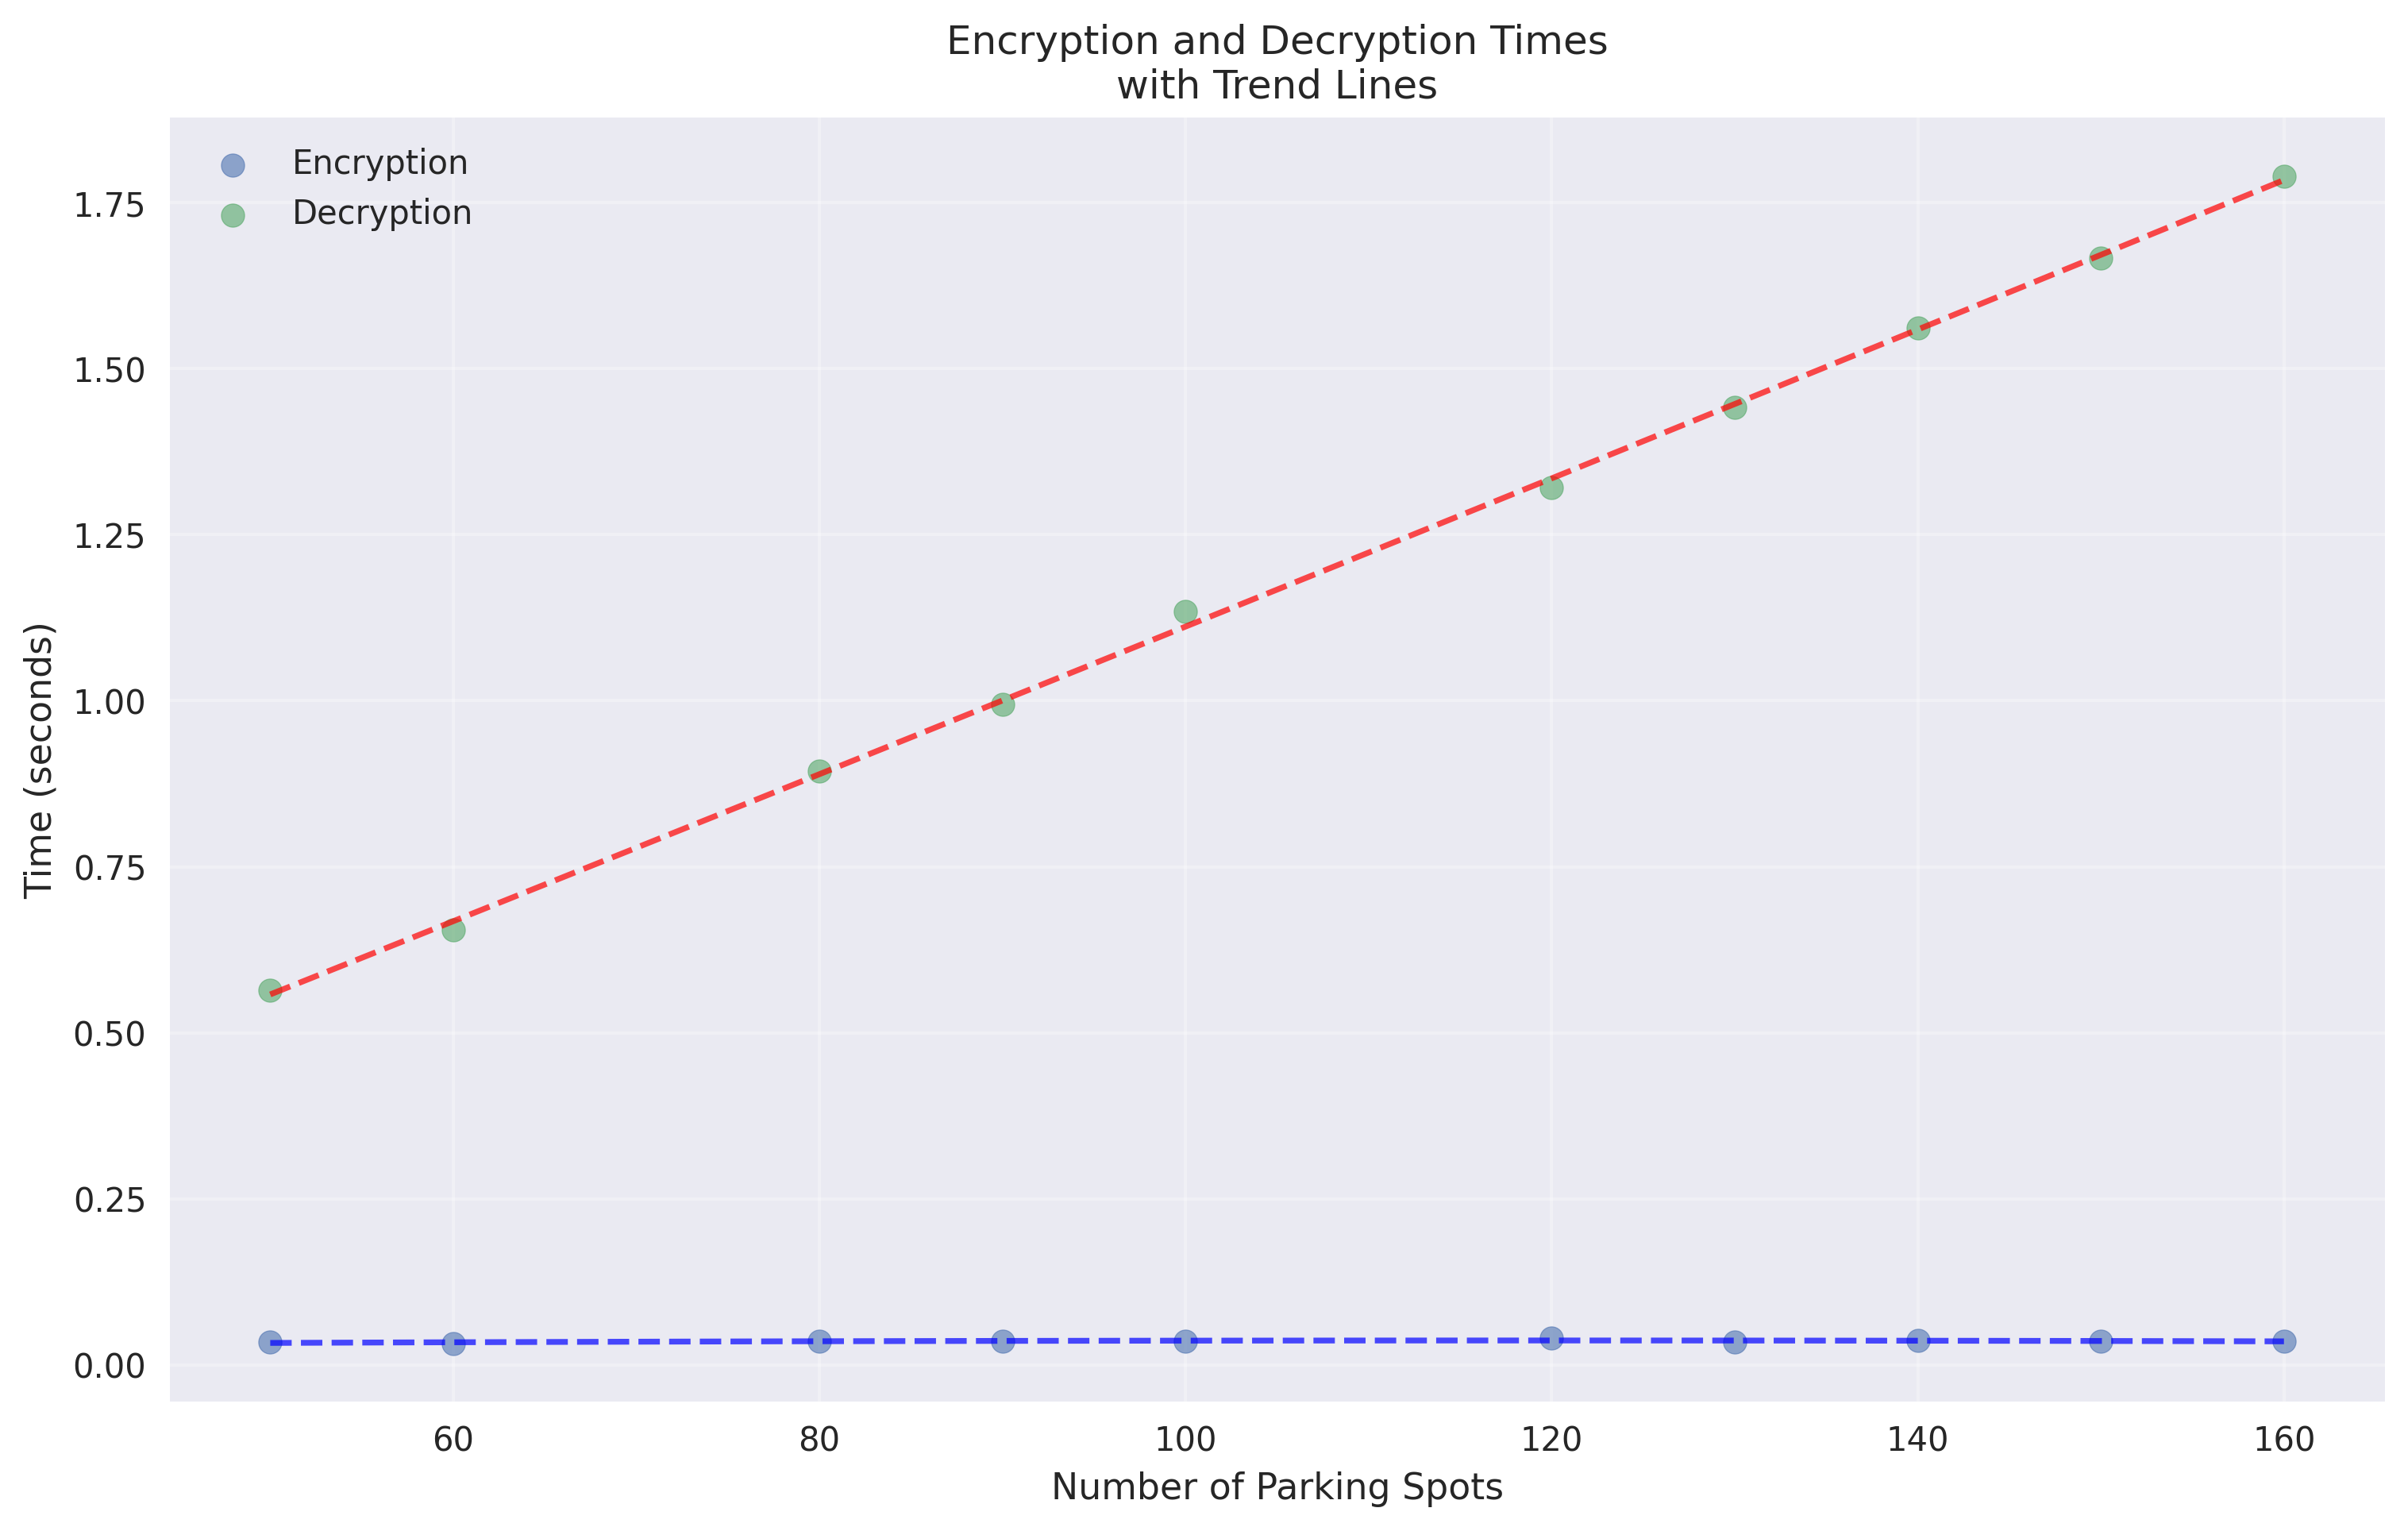
\includegraphics[width=\columnwidth]{img/crypto_times.png}
    \caption{Visualization of the Encryption and Decryption time using HE}
    \label{fig:testing-enc}
\end{figure}

The test begins with the generation of the parameters for the homomorphic encryption scheme, followed by the key generation. The code snippet in Listing \ref{lst:enc-decrypt} shows the code used to encrypt and decrypt the client position.
% add the code to encrypt
\lstset{frame=tb,
  language=python,
  aboveskip=3mm,
  belowskip=3mm,
  showstringspaces=false,
  columns=flexible,
  basicstyle={\small\ttfamily},
  numbers=none,
  numberstyle=\tiny\color{gray},
  keywordstyle=\color{blue},
  commentstyle=\color{dkgreen},
  stringstyle=\color{magenta},
  breaklines=true,
  breakatwhitespace=true,
  tabsize=3
}

\newpage

\begin{lstlisting}[language=python, caption={Encryption and Decryption of the client position}, label={lst:enc-decrypt}]
parameters = CCParamsBGVRNS()
parameters.SetPlaintextModulus(65537)
parameters.SetMultiplicativeDepth(2)

crypto_context = GenCryptoContext(parameters)
crypto_context.Enable(PKESchemeFeature.PKE)
crypto_context.Enable(PKESchemeFeature.KEYSWITCH)
crypto_context.Enable(PKESchemeFeature.LEVELEDSHE)

keypair = crypto_context.KeyGen()
crypto_context.EvalMultKeyGen(keypair.secretKey)
\end{lstlisting}


The next step is to compute the distances between the client position and the parking spots. The code snippet in Listing \ref{lst:compute-distances} shows the code used to compute the distances using the homomorphic encryption scheme.

\begin{lstlisting}[caption={Computing distances using Homomorphic Encryption}, label={lst:compute-distances}]
# Encrypt the client position
query_plaintext = crypto_context.MakePackedPlaintext([query_encoded])
query_ciphertext = crypto_context.Encrypt(keypair.publicKey, query_plaintext)

# Process each spot
spots = parking_system.get_spots()

for spot_id, spot in spots.items():
    # Create plaintext for the spot's encoded position
    spot_plaintext = crypto_context.MakePackedPlaintext([spot['encoded_pos']])
    
    # Homomorphic subtraction to check if positions match
    diff_ciphertext = crypto_context.EvalSub(query_ciphertext, spot_plaintext)
                
    diff_plaintext = crypto_context.Decrypt(keypair.secretKey, diff_ciphertext)

\end{lstlisting}

This two sections from the original codebase showcase how the encryption distance calculation works. The full code contains additional logic for handling metrics and logging.

In order to have a fair comparison with other common encryption standards, I made the test run in parallel by multi-processing on the same machine. This refiniment made the test more realistic, as in a real-world scenario, multiple clients would be sending requests to the server at the same time with multiple parking spots (subscribers).

\begin{figure}[h]
    \centering
    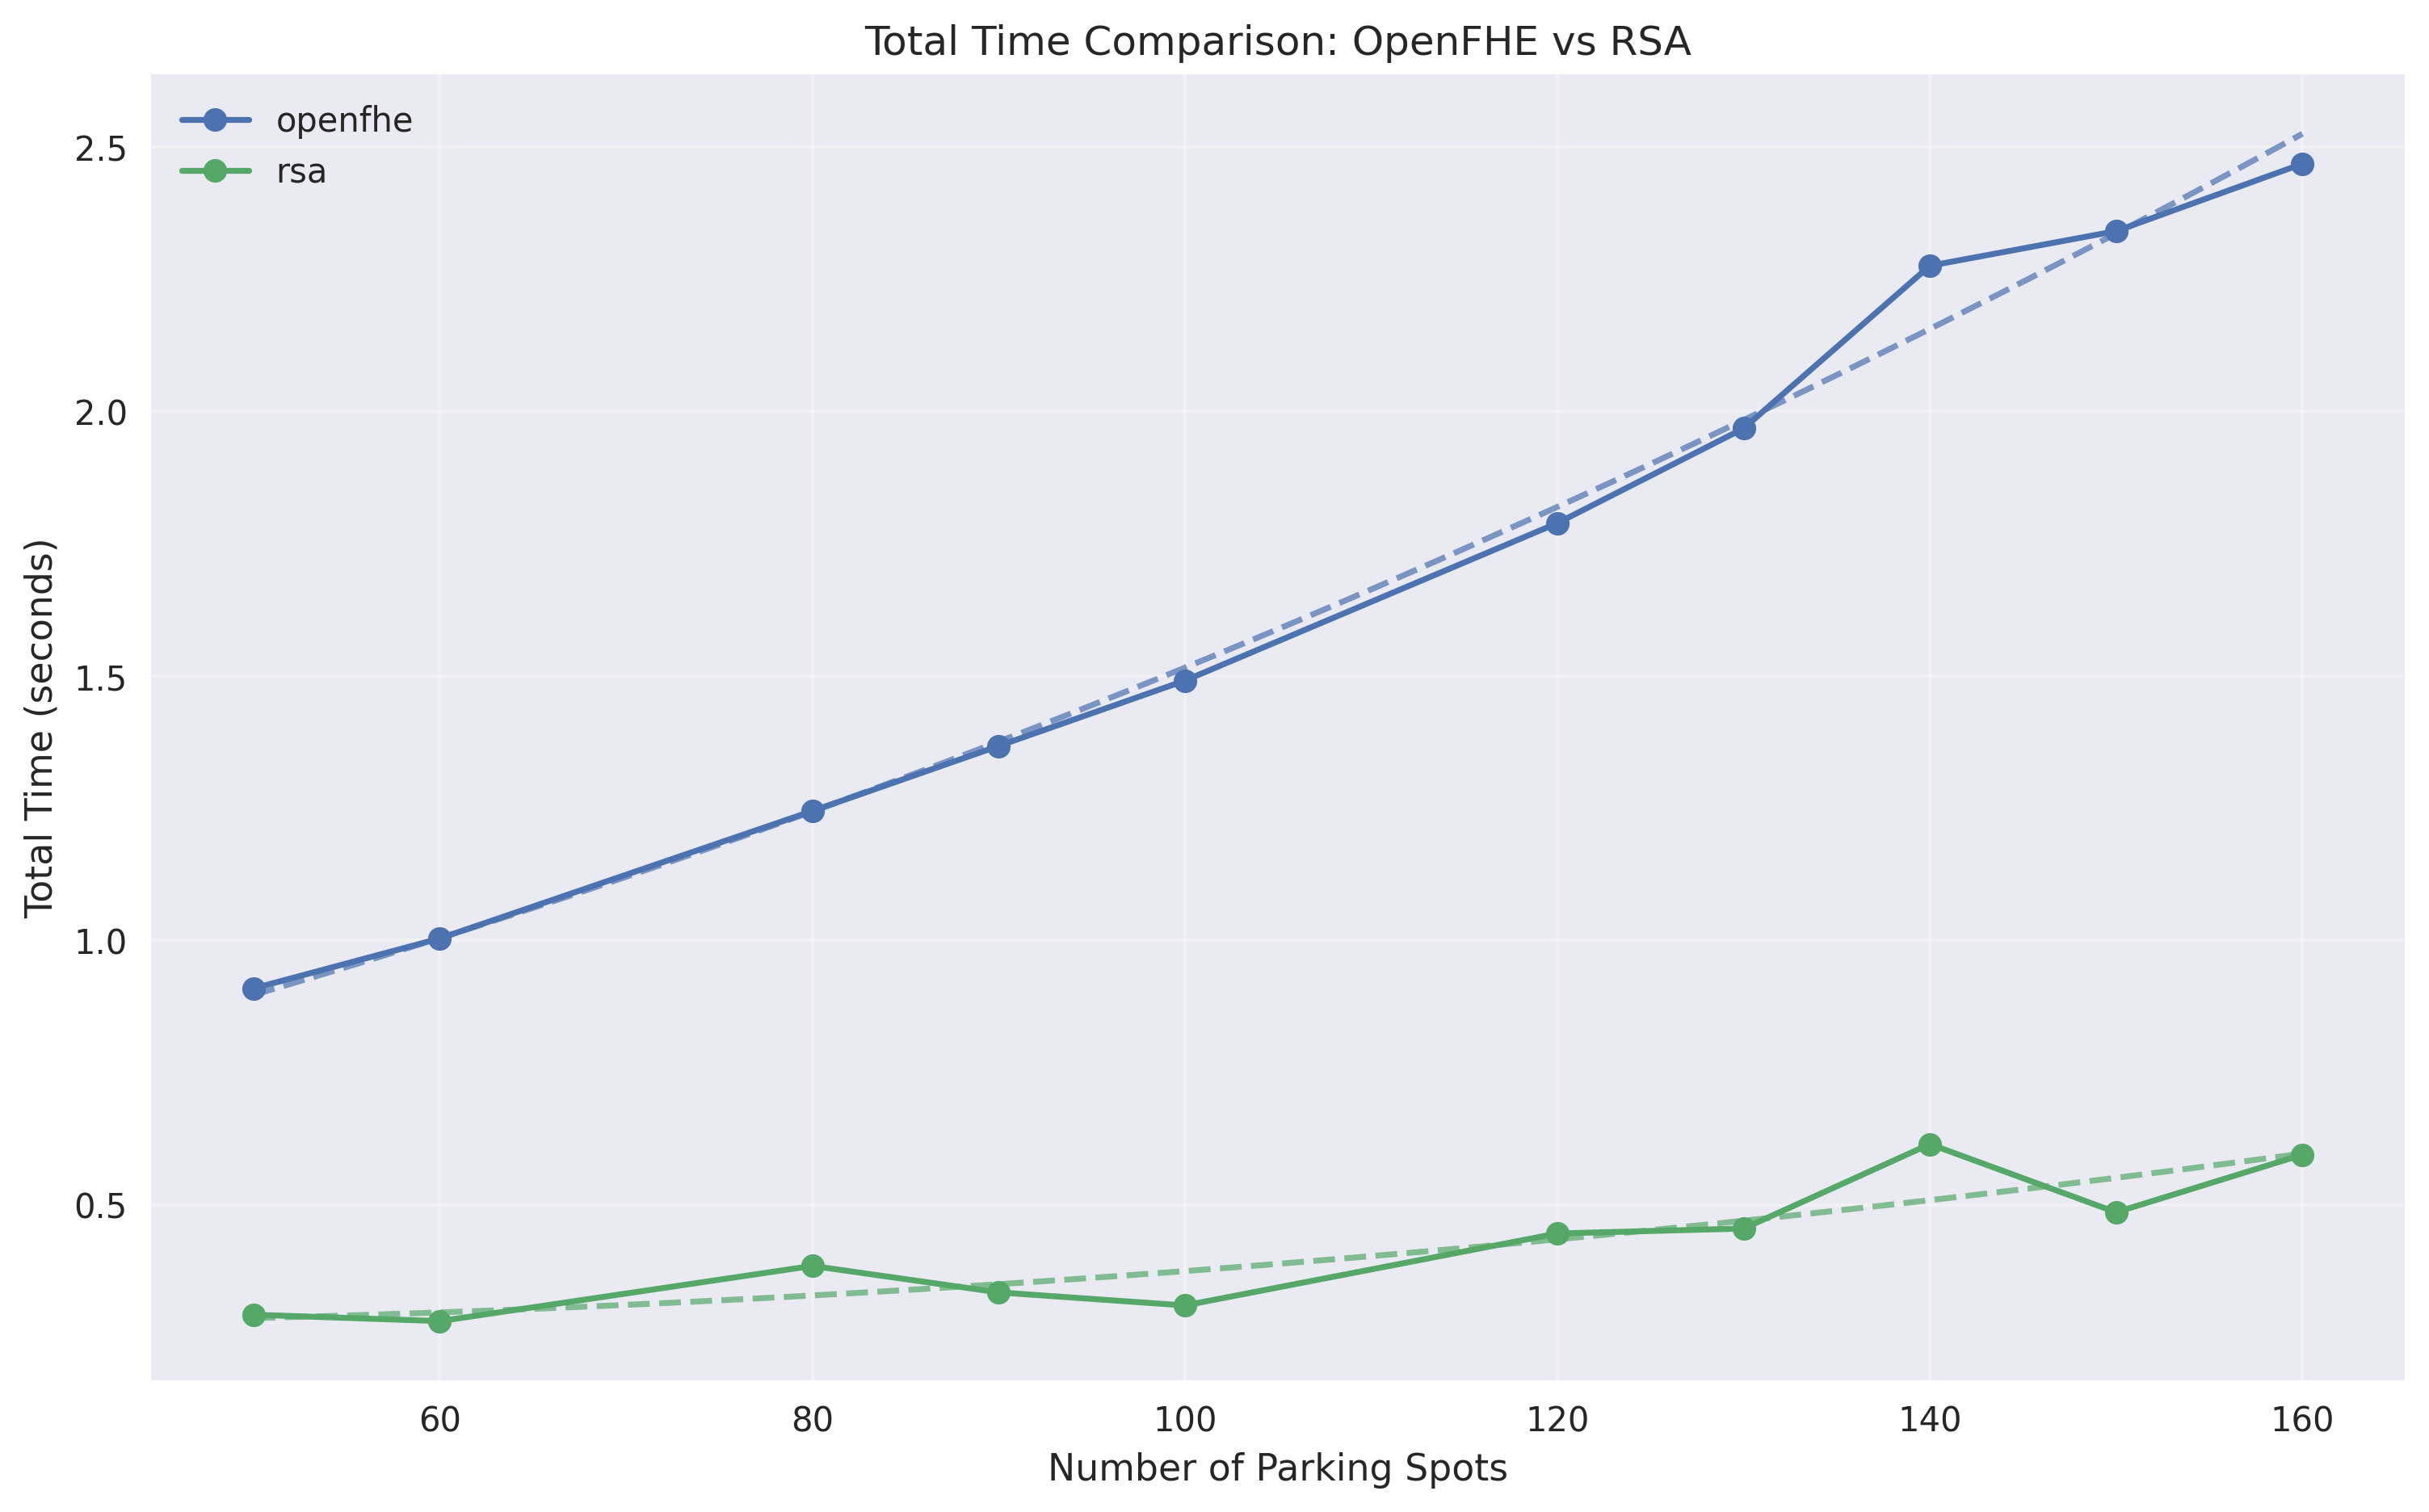
\includegraphics[width=12.5cm,height=9cm]{img/total_time_comparison.png}
    \caption{Comparison between RSA and HE for encryption and decryption}
    \label{fig:he-vs-rsa}
\end{figure}

The overall time performance of the protocol is shown in \cref{fig:he-vs-rsa} confirms that the HE standard has some overhead compared to the RSA standard, but it is still acceptable for a real-world scenario. The main difference between the two encryption standards is that, with the symmetric encryption, the server, after decrypting the client position, is much faster in computing the distances, as it can be achieved in a couple of instructions.

Although the homomorphic encryption needs to perform a simple subtraction, it is still slower, as values need to be packed to match HE standards \ref{lst:compute-distances}.

It also worth to mention the way the distances are computed in our protocol. Firstly, we need to encode the GPS coordinates into a grid-like structure. This operation is essential to ensure that we are considering small areas instead of points \cref{lst:distance-computation}. Then we apply a unique encoding to the grid coordinates, transforming them from a two-dimensional grid into a one-dimensional z-order curve. By having a single integer representation we can perform easily the distance.

\begin{lstlisting}[caption={Distance computation using z-order encoding}, label={lst:distance-computation}]
def calculate_grid_sizes_for_radius(radius_meters, max_lat, min_lat, max_lon, min_lon):
    radius_km = radius_meters / 1000.0
    lat_span = max_lat - min_lat
    lon_span = max_lon - min_lon
    
    # Latitude: fixed ~111.32 km/degree
    lat_cells = int(lat_span / (radius_km / 111.32))
    
    # Longitude: depends on latitude
    mean_lat = math.radians((max_lat + min_lat) / 2)
    lon_cells = int(lon_span / (radius_km / (111.32 * math.cos(mean_lat))))
    
    return lat_cells, lon_cells  # Return separate sizes

def normalize_gps(lat, lon, lat_cells=None, lon_cells=None, edge_meters=500, max_lat=44.499194, min_lat=44.492307, max_lon=11.363250, min_lon=11.325319):

    if lat_cells is None or lon_cells is None:
        lat_cells, lon_cells = calculate_grid_sizes_for_radius(edge_meters, max_lat, min_lat, max_lon, min_lon)
    
    grid_x = int((lat - min_lat) / (max_lat - min_lat) * lat_cells)
    grid_y = int((lon - min_lon) / (max_lon - min_lon) * lon_cells)
    
    return grid_x, grid_y
\end{lstlisting}

To compute the z-order encoding, we use a straightforward approach that interleaves the bits of the x and y coordinates. The code snippet in Listing \ref{lst:z-order-encoding} shows how we compute the z-order encoding for the grid coordinates.

\begin{lstlisting}[caption={Z-order encoding for grid coordinates}, label={lst:z-order-encoding}]
def interleave_bits(x, y):
    """
    Interleave the bits of x and y to create a Morton code.
    x and y should be non-negative integers, each limited to 16 bits.
    """
    # Ensure inputs are within 16-bit range
    x = min(x, 0xFFFF)
    y = min(y, 0xFFFF)
    
    # Convert to binary and pad with zeros to 16 bits
    x_bin = format(x, '016b')
    y_bin = format(y, '016b')
    
    # Interleave the bits
    result = ''
    for i in range(16):
        result += x_bin[i] + y_bin[i]
    
    return int(result, 2)
\end{lstlisting}


There are also other approaches to compute distances between two encrypted points\cite{ibarrond2022hedistancetricks}, as mentioned for the methods in \cref{sec:background-distances}:
\begin{itemize}
    \item \textbf{Cosine similarity:} This can be resolved by normalizing the vectors, i.e., $\mathbf{x}' = \mathbf{x} / \|\mathbf{x}\|$ and $\mathbf{y}' = \mathbf{y} / \|\mathbf{y}\|$, encrypting $\mathbf{x}'$ and $\mathbf{y}'$, and then performing a simple scalar product: $\sum_i x'_i y'_i$.
    
    \item \textbf{Euclidean Distance:} would require a square root operation.\\
    Instead we use the \textbf{Squared Euclidean Distance} instead:
    $
    \mathrm{SED}(\mathbf{x}, \mathbf{y}) = \sum_i (x_i - y_i)^2
    $
    
    \item \textbf{Manhattan Distance:} in this case it is also require computing the absolute value.\\
    If you encrypt only binary values (i.e., $\hat{\mathbf{x}}, \hat{\mathbf{y}}$ such that $\hat{x}_i, \hat{y}_i \in \{0,1\}$ for all $i$), you can reformulate:
    $
    \mathrm{MD}(\hat{\mathbf{x}}, \hat{\mathbf{y}}) = \sum_i (\hat{x}_i - \hat{y}_i)^2 = \mathrm{HD}(\hat{\mathbf{x}}, \hat{\mathbf{y}})
    $
    which is the \textbf{Hamming Distance} . For non-binary vectors, you can at least compute the \textbf{Squared Manhattan Distance}
    $
    \mathrm{SMD}(\mathbf{x}, \mathbf{y}) = \sum_i (x_i - y_i)^2
    $
    but this is missing a square root to recover the standard Manhattan distance.
    
\end{itemize}

Rounding off, all of these methods have the problems of relying on calculations on floating point numbers, which is not ideal for homomorphic encryption. Another way could be to normalize the coordinates to integers, with a fixed order of magnitude, but it is not worth the effort, as the z-order encoding is already a good solution for this problem.

